% Лабораторная работа по АСиСу № 1
% Михедов Константин Константинович

% Тип документа: статья, на бумаге А4
\documentclass[a4paper]{article}

% Подключение сторонних tex файлов 
\usepackage{import}


% Основные данные - ВУЗ, факультет, город...
\import{./../../stuff/tex}{config.tex}

% Подключение необходимых зависимостей
\import{./../../stuff/tex/settings}{packages.tex}
% Настройка подключенных пакетов
\import{./../../stuff/tex/settings}{preferences.tex}


% Шаблон титульной страницы 
\import{./../../stuff/tex/templates}{title.tex}
% Упрощенный блок "выполнил"
\import{./../../stuff/tex/templates}{sign1.tex}
% Макрос для содержания
\import{./../../stuff/tex/templates}{toc.tex}

% Определяем название документа
\title{
  Лабораторная работа №1 по курсу \\
  <<Компьютерный практикум <<Админимтрирование систем и сетей>>  
}
% Отключаем отображение правительства
\renewcommand{\government}{}
% Отключаем сокращенное нзавание университета
\renewcommand{\subuniversity}{}
% Указываем преподавателя
\renewcommand{\shortteachername}{Зудин Д.Е.}


% Путь до внешних изображений
\graphicspath{ {./figures/}}


% Основной текст работы
\begin{document}
  \templatedtitlepage
  
  \toc
  \section{Ход работы}

  \subsection{Настройка рабочего окружения}

  Для выполнения данной лабораторной работы я использовал персональный компьютер,
  с установленной на нем операционной системой Arch-Linux (с последними обновлениями).
  Чтобы приступить к основной части работы, необходимо установить неодостающие пакеты при 
  помощи следующей команды:

  \begin{minted}{bash}
    sudo pacman -S wireshark-qt net-tools bind wget
  \end{minted}

  Пакет \textit{net-tools} соедржит в себе утилиту ifconfig, а \textit{bind} - nslookup, которые
  понадобятся для получения информации о системе и выполнения DNS-запросов.

  \subsection{Получение IP адреса}

  Для того, чтобы узнать IP компьютера, необходимо узнать, как сетевой интерфейс используется
  для подключения к Интернету. Посмотрим список и состояние имеющихся сетевых интерфейсов при 
  помощи утилиты \textit{nmcli}:

  \begin{figure}[H]
    \centering
    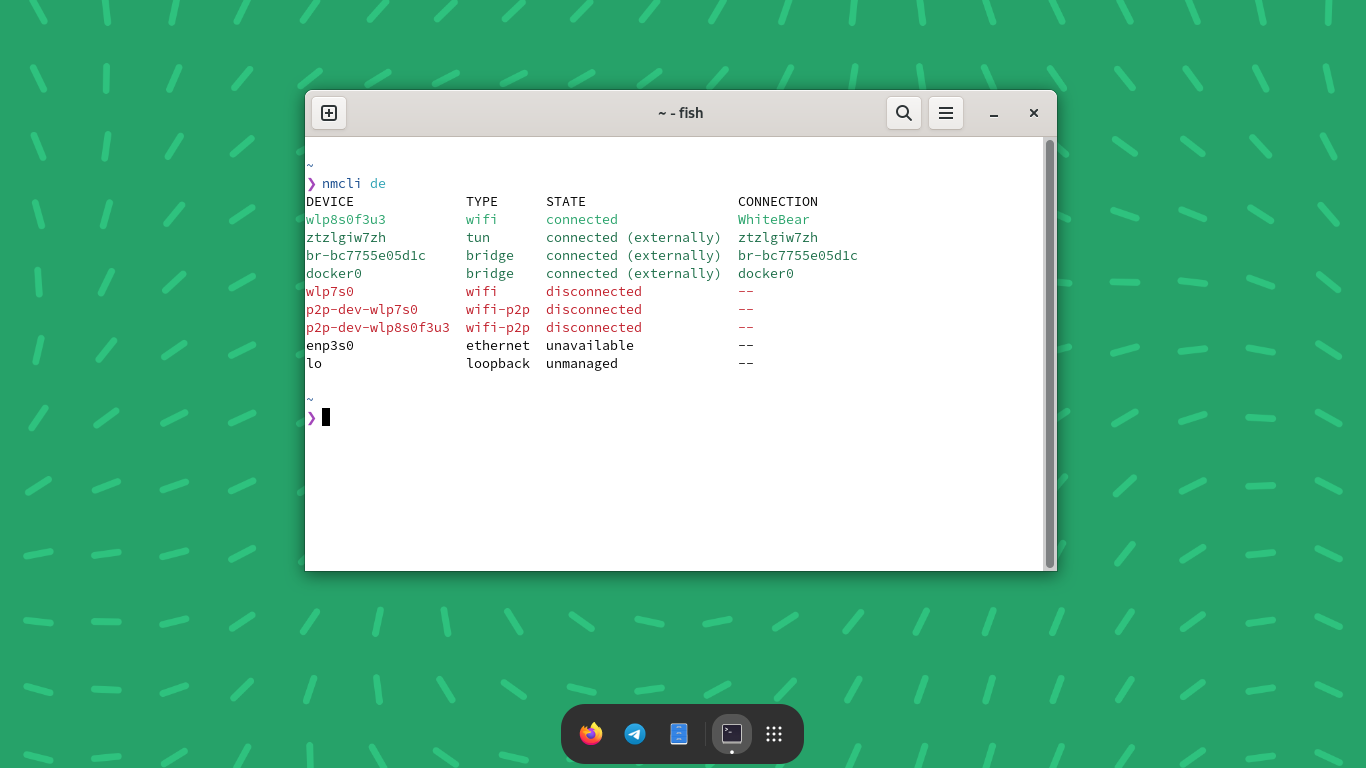
\includegraphics[width=1.0\textwidth]{01_0001}
    \caption{Информация о сетевых интерфейсах}
    \label{img:0001}
  \end{figure}

  Из вывода команды (рис. \ref{img:0001} на стр. \pageref{img:0001}) можно понять, что для соединения с сетью происходит при помощи WiFi:
  устройство \textit{wlp8s0f3u3} подключено к беспроводной сети \textit{WhiteBear}.
  Далее необходимо подробнее узнать об этом устройстве,
  для этого воспользуемся ранее установленной утилитой \textit{ifconfig}:

  \begin{figure}[H]
    \centering
    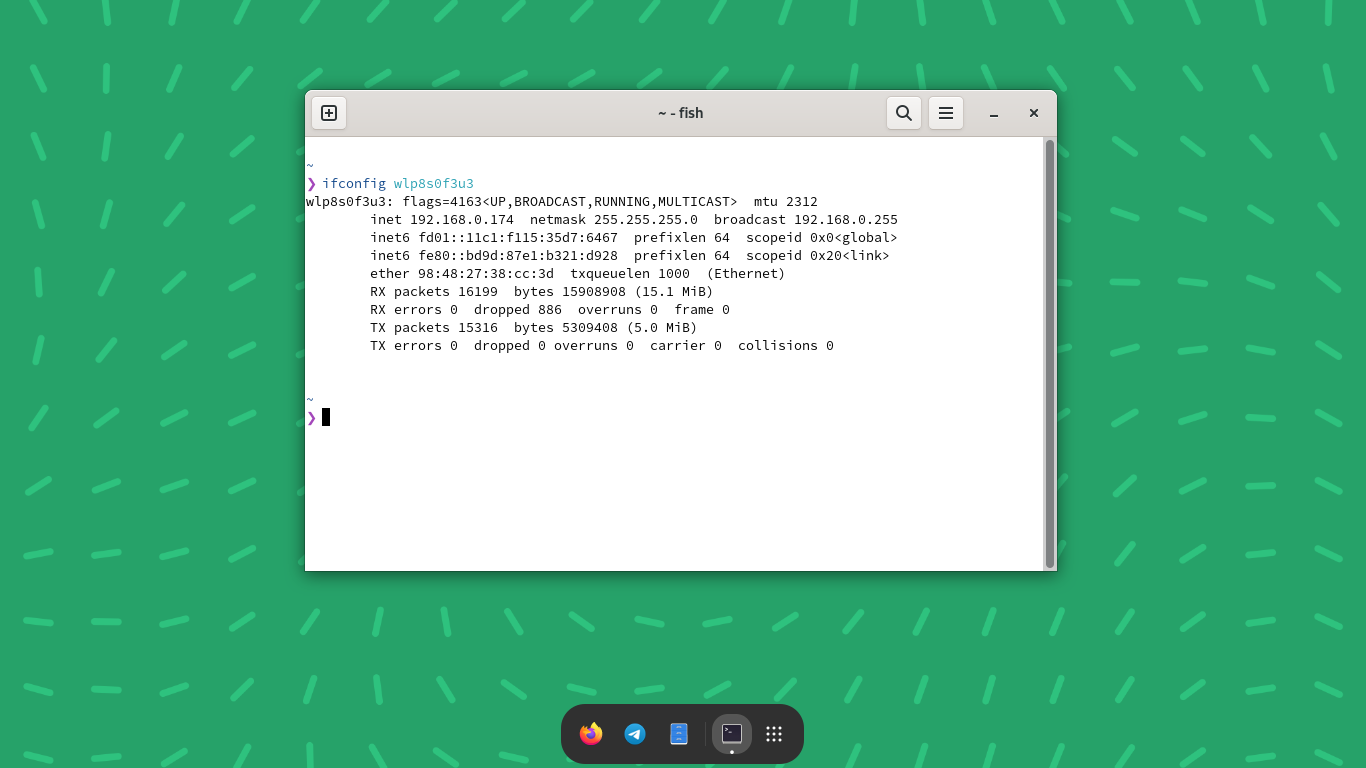
\includegraphics[width=1.0\textwidth]{01_0002}
    \caption{Информация об устройстве wlp8s0f3u3}
    \label{img:0002}
  \end{figure}

  Благодаря полученным данным становиться ясно, что IPv4 устройства - 192.168.0.174 (рис. \ref{img:0002} на стр. \pageref{img:0002}).

  \subsection{Старт захвата пакетов}

  Для запуска \textit{Wireshark} требуются дополнительные разрешения, чтобы их получить, добавим
  текущего пользователя в группу wireshark:

  \begin{minted}{bash}
    sudo usermod -a -G wireshark ${whoami}
  \end{minted}  

  Теперь права на перехват пакетов получены, запускаем \textit{Wireshark} и запускаем сниффинг
  на ранее полученном устройстве, дважды щелкнув по нему мышью (рис. \ref{img:0004} на стр. \pageref{img:0004}):

  \begin{figure}[H]
    \centering
    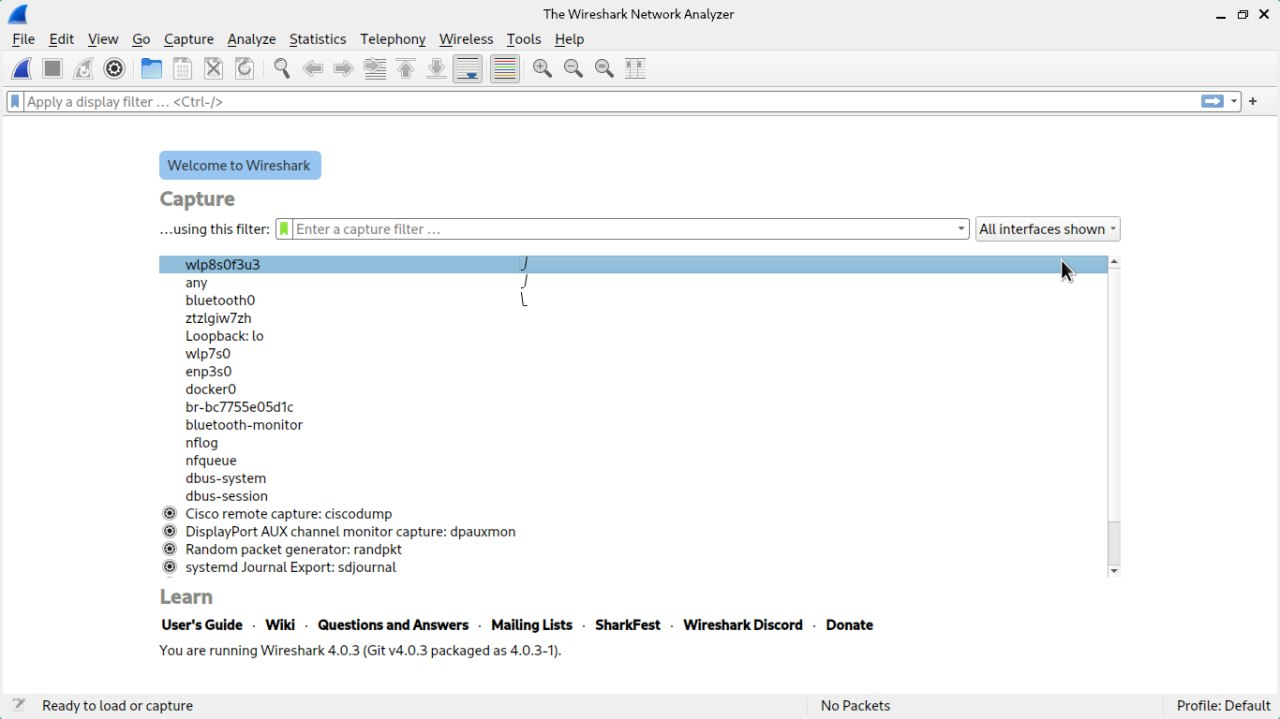
\includegraphics[width=1.0\textwidth]{01_0004}
    \caption{Главное окно Wireshark}
    \label{img:0004}
  \end{figure}

  \subsection{Отлавливание ICMP-пакетов}

  В качестве ресурса, на который будут отправлены icmp пакеты, был выбран \textit{ya.ru}.
  Для начала узнаем IPv4 ресурса при помощи \textit{nslookup}, затем отправим 3 пакета при 
  помощи утилиты \textit{ping} (рис. \ref{img:0005} на стр. \pageref{img:0005}).

  \begin{figure}[H]
    \centering
    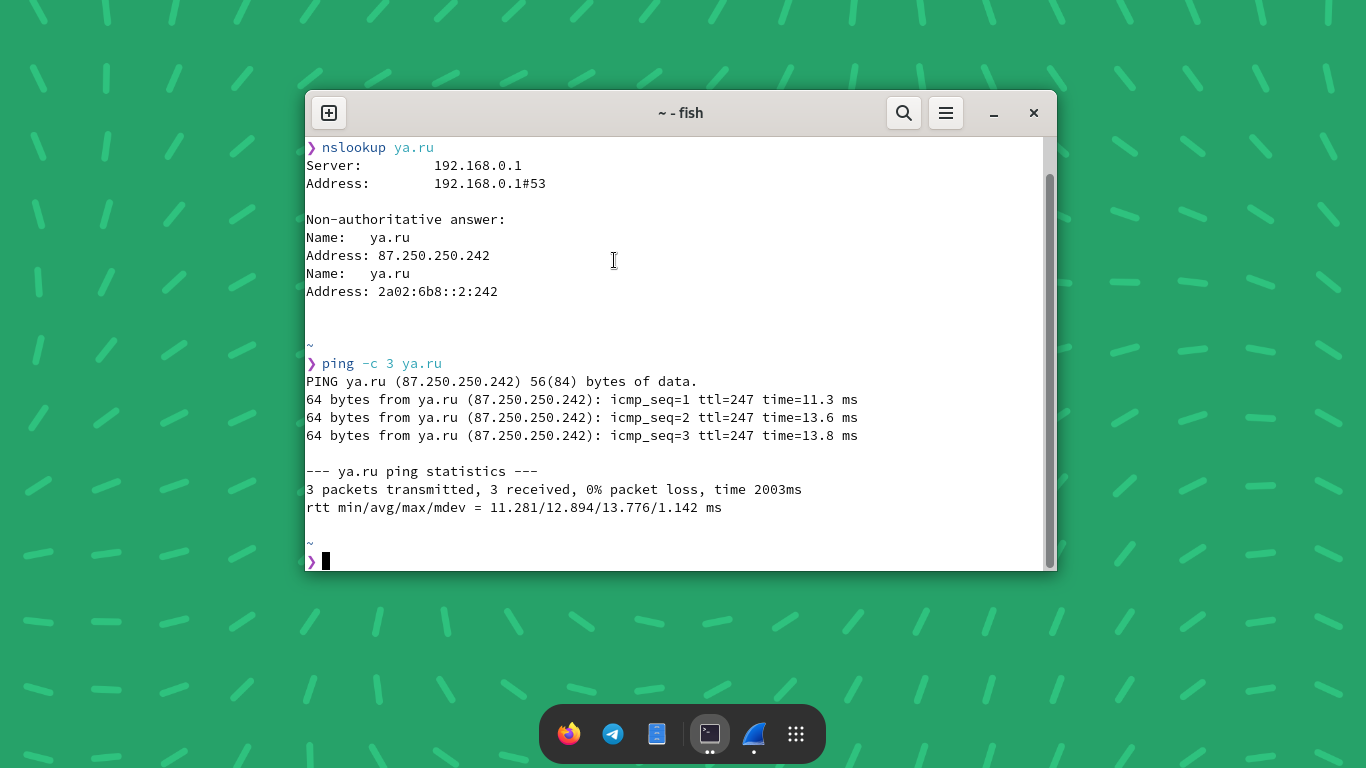
\includegraphics[width=0.9\textwidth]{01_0005}
    \caption{Ping ресурса ya.ru}
    \label{img:0005}
  \end{figure}

  Из вывода команд видно, что IPv4 ресурса - 87.250.250.242. Найдем в \textit{Wireshark}
  icmp пакеты, отправленные по на данный адрес:

  \begin{figure}[H]
    \centering
    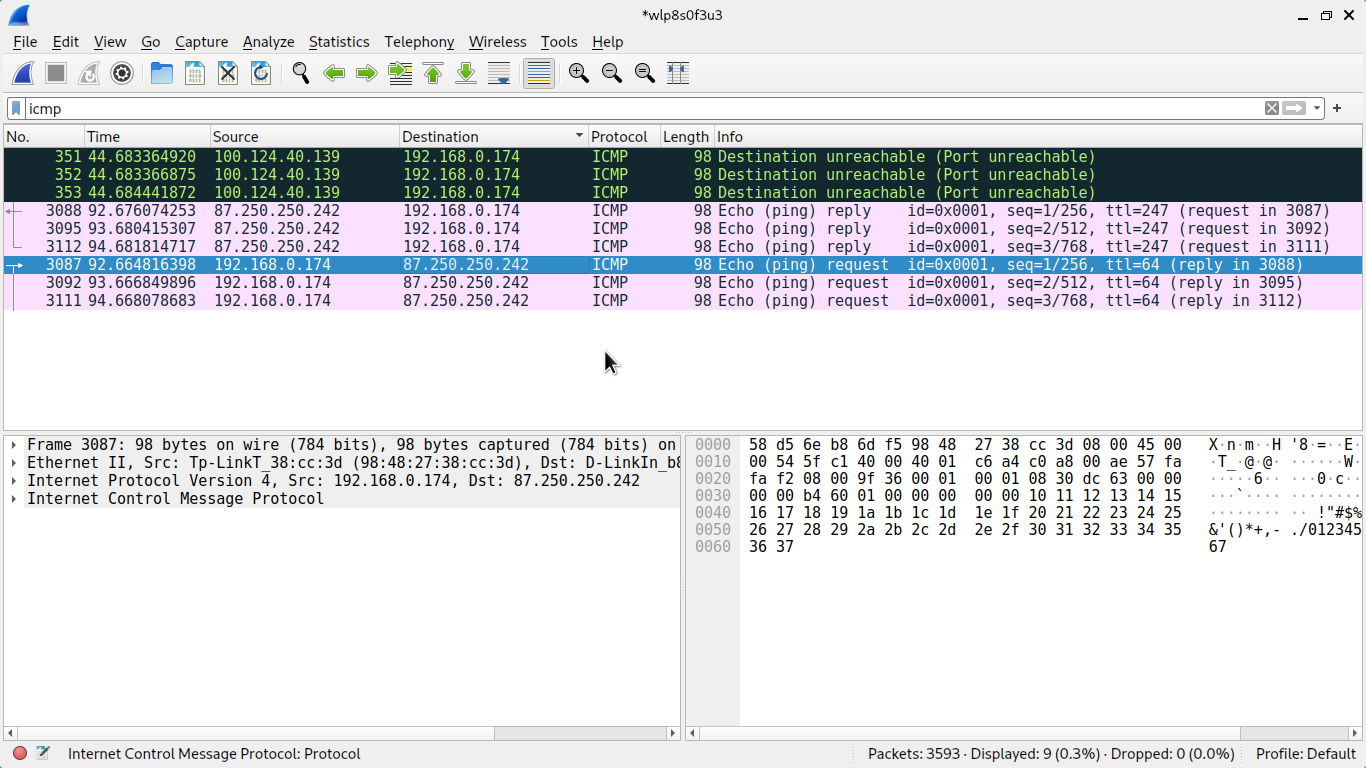
\includegraphics[width=1.0\textwidth]{01_0006}
    \caption{Перехваченные ICMP пакеты}
    \label{img:0006}
  \end{figure}

  \textit{Wireshark} захватил ровно 3 ICMP пакета, отправленных на ya.ru (рис. \ref{img:0006}
  на стр. \pageref{img:0006}), а это как раз столько, сколько было указано команде \textit{ping}.
  IPv4 отправителя также полностью совпадает с адресом компьютера, который был получен ранее.

  \subsection{Перехват HTTP}

  Для перехвата HTTP запросим файл \href{http://info.cern.ch/hypertext/WWW/TheProject.html}{TheProject.html} при 
  помощи утилиты \textit{wget} (рис. \ref{img:0007} на стр. \pageref{img:0007}), затем отфильтруем захваченные \textit{Wireshark} пакеты по 
  протоколу HTTP. Можно увидеть два перехваченных HTTP пакета - GET запрос от клиента к серверу
  (рис. \ref{img:0008} на стр. \pageref{img:0008}) и ответ сервера на этот запрос
  (рис. \ref{img:0009} на стр. \pageref{img:0009}).

  \begin{figure}[H]
    \centering
    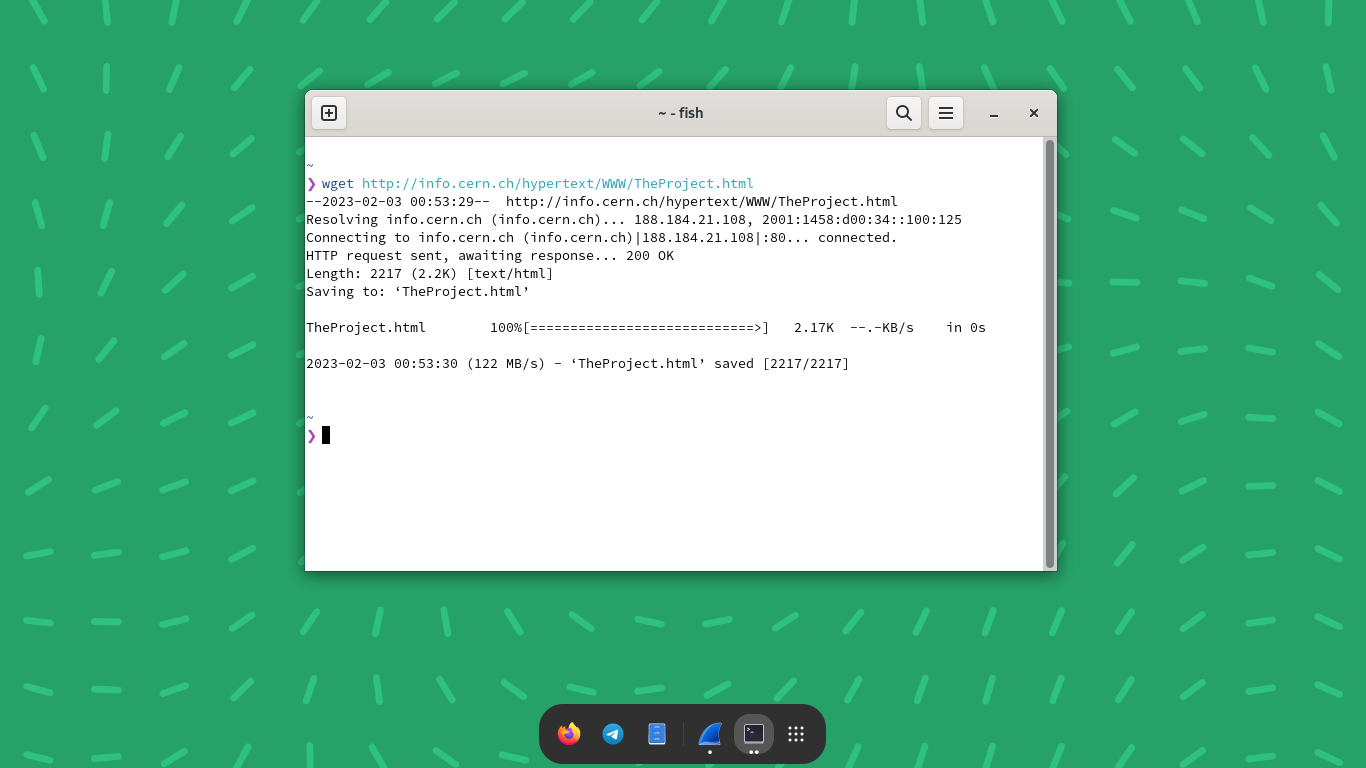
\includegraphics[width=1.0\textwidth]{01_0007}
    \caption{Получение HTML странички через HTTP}
    \label{img:0007}
  \end{figure}

  \begin{figure}[H]
    \centering
    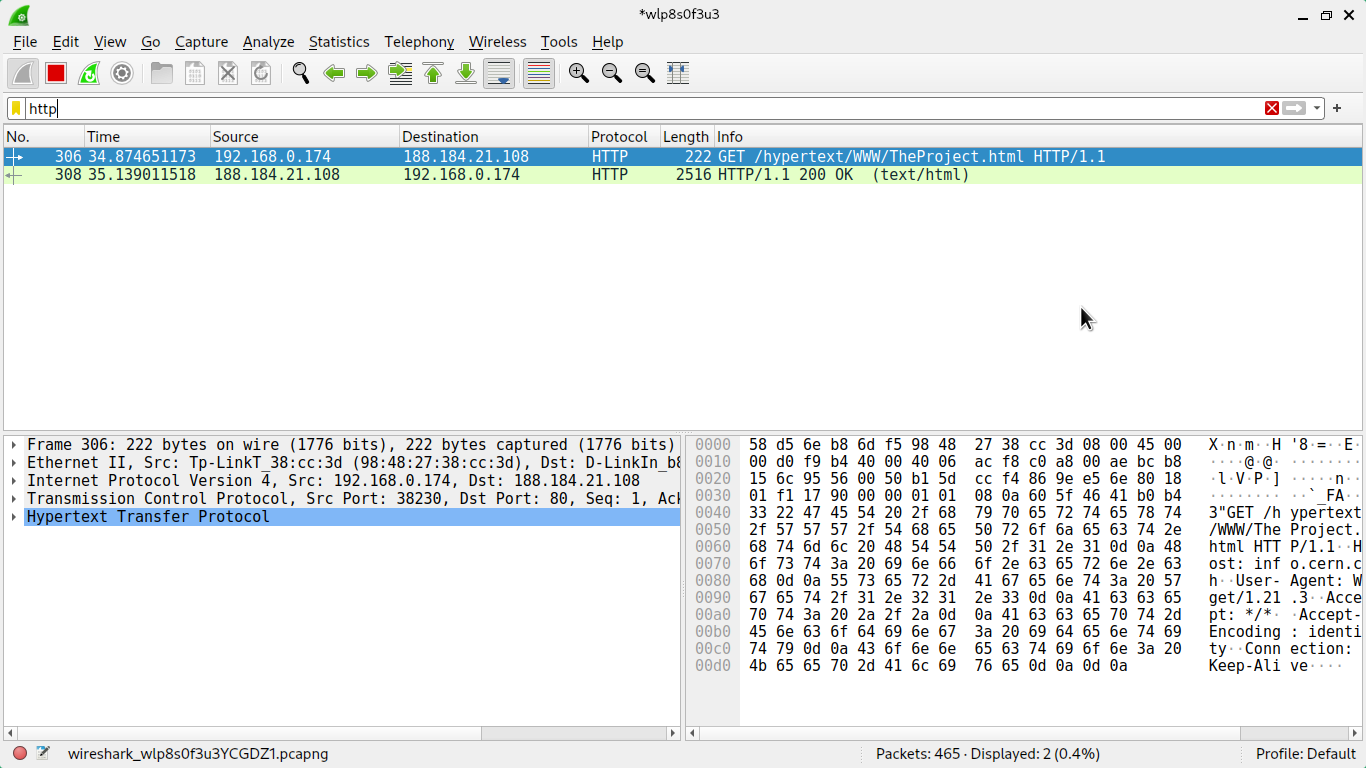
\includegraphics[width=1.0\textwidth]{01_0008}
    \caption{Перехваченный HTTP GET запрос}
    \label{img:0008}
  \end{figure}

  \begin{figure}[H]
    \centering
    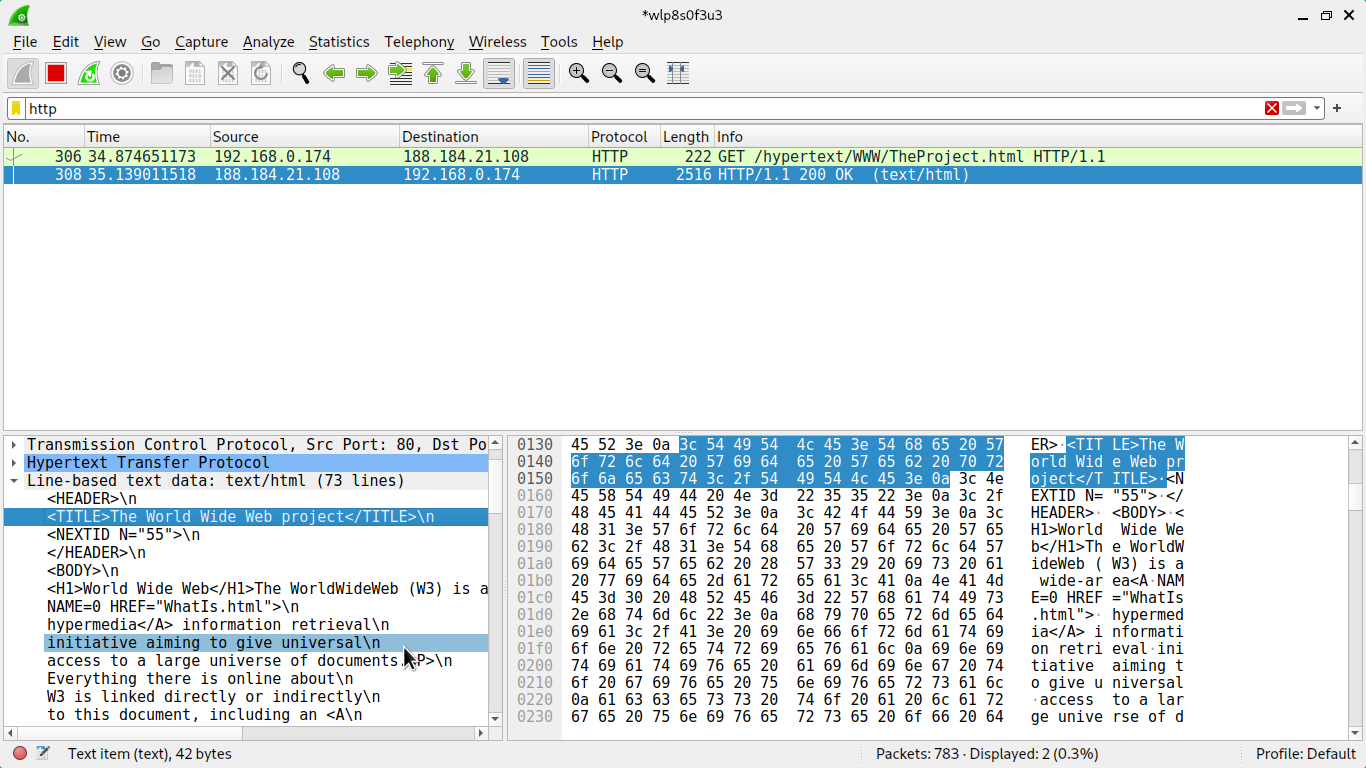
\includegraphics[width=1.0\textwidth]{01_0009}
    \caption{Перехваченный ответ HTTP сервера}
    \label{img:0009}
  \end{figure}

  В теле запроса можно увидеть имя запрошенного нами ресурса, а в ответе можно заметить, что
  атрибут \textit{title} полученной html странички <<The World Wide Web project>>, что 
  полностью совпадает с заголовком, который отобразит браузер при отображение данной страницы
  (рис. \ref{img:0010} на стр. \pageref{img:0010}).

  \begin{figure}[H]
    \centering
    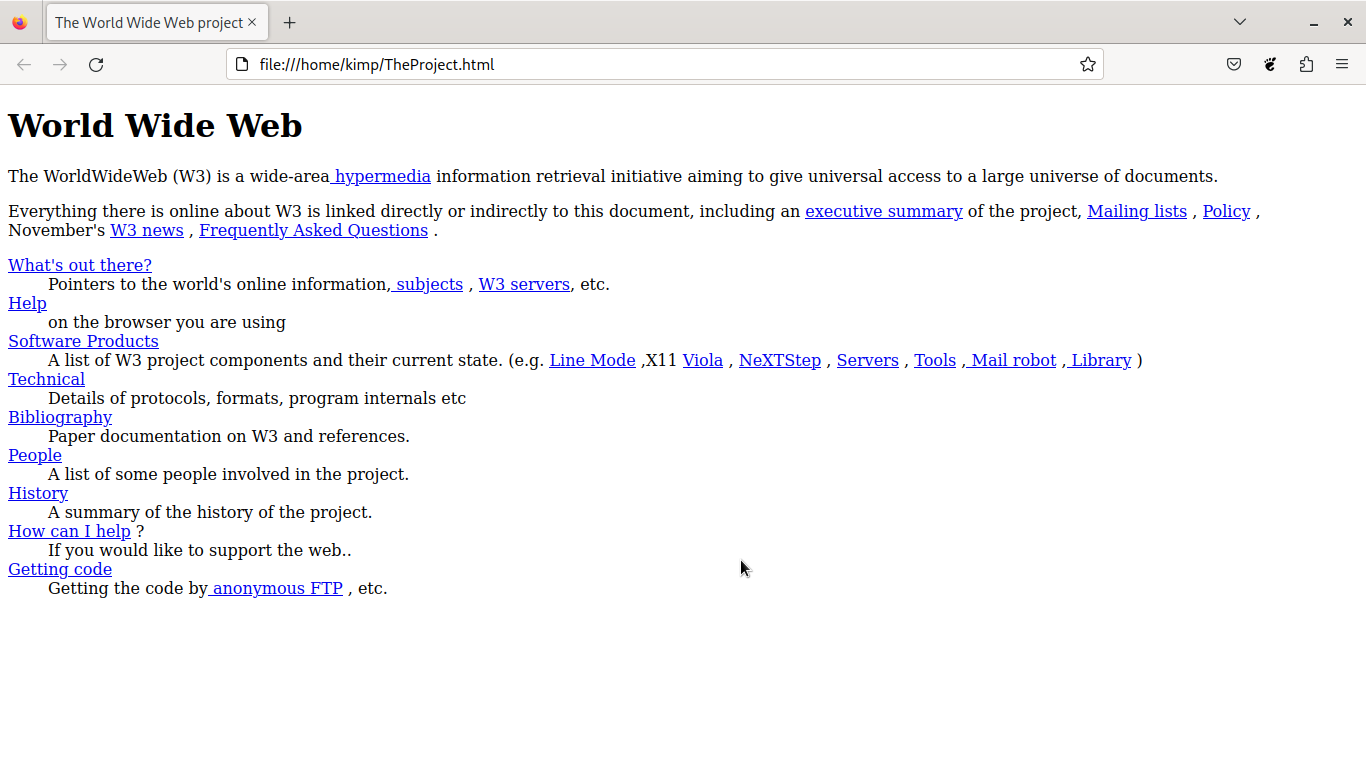
\includegraphics[width=0.9\textwidth]{01_0010}
    \caption{Полученная html страница}
    \label{img:0010}
  \end{figure}

  \section{Вывод}

  В ходе данной лабораторной работы мне удалось научитсья перехватывать отправленные и
  полученный пакеты при помощи \textit{Wireshark}, разобраться со встроенным в данное 
  ПО фильтром, улучшить свои навыки работы с терминалом.
\end{document}
